\documentclass[a4paper,11pt]{article}
\usepackage[polish]{babel}
\usepackage[OT4]{fontenc}
\usepackage[utf8]{inputenc}
\usepackage{graphicx}

\usepackage{epstopdf}




\date{21/03/2014}


%opening
\title{PAMSI -- testowanie algorytmów sortowania}
\author{Piotr Wilkosz}



\begin{document}

\maketitle



\section{Wstęp}
Celem ćwiczenia było przetestowanie złożoności obliczeń algorytmów. Do testowania zostały wybrane 3 z puli algorytmów na ocenę bardzo dobrą:
\begin{itemize}
 \item Quick-sort (sortowanie szybkie)
 \item Heap-sort (sortowanie przez kopcowanie)
 \item Merge-sort (sortowanie przez scalanie)
\end{itemize}

\section{Wyniki pomiarów}

\begin{enumerate}
 \item Quick-sort:
 \begin{figure}[!h]
\centering
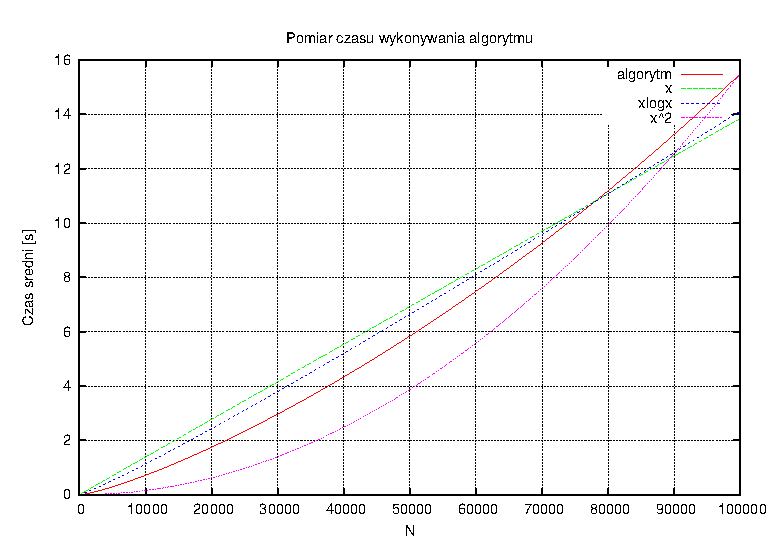
\includegraphics[width=0.8\textwidth]{../prj/wykres7.eps}
\caption{Test nr 1}
\label{Test nr 1}
\end{figure} 
\newpage
 \item Heap-sort:
 \begin{figure}[!h]
\centering
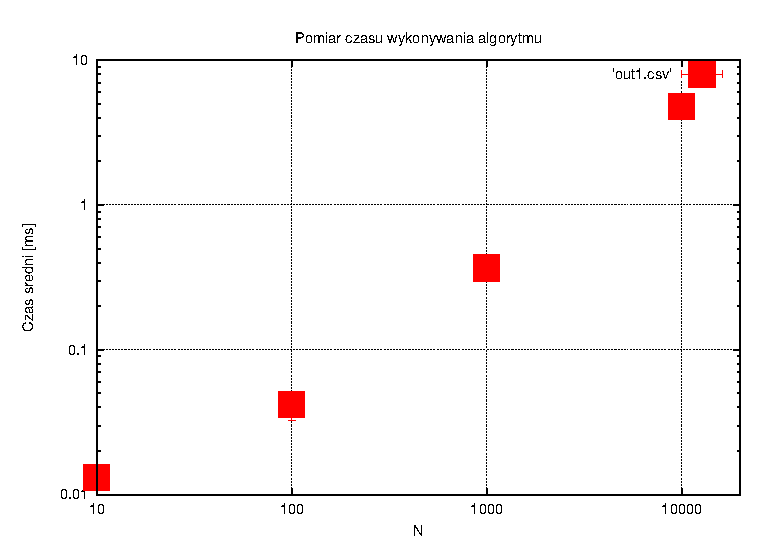
\includegraphics[width=0.8\textwidth]{../prj/wykres8.eps}
\caption{Test nr 2}
\label{Test nr 2}
\end{figure} 
\item Mergesort

 \begin{figure}[!h]
\centering
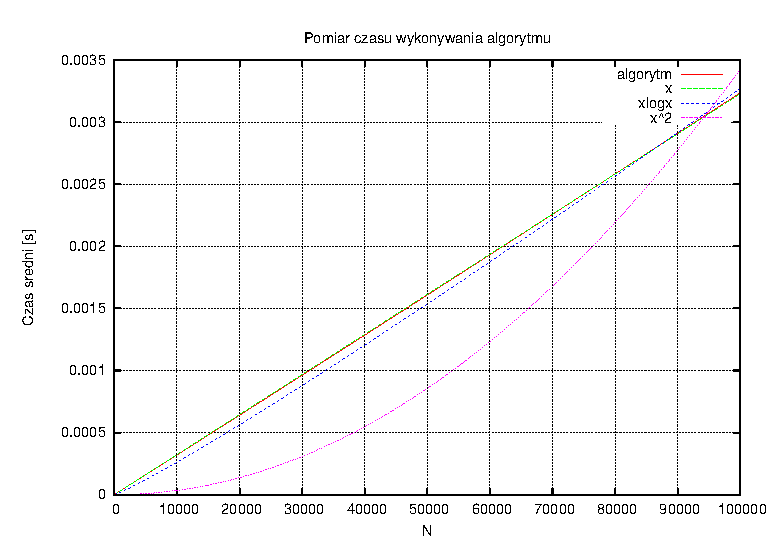
\includegraphics[width=0.8\textwidth]{../prj/wykres9.eps}
\caption{Test nr 3}
\label{Test nr 3}
\end{figure} 

\section{Wnioski}
\begin{itemize}
 \item Sortowanie szybkie, spośród powyższych, okazało się najłatwiejsze w implementacji.
 \item Złożoność obliczeniową powyższych algorytmów szacuje się na $ O(n logn) $
 \item Algorytm sortowania szybkiego okazał się najszybszy, co nie oznacza, że jest on niezawodny. Istnieje taka możliwość, gdzie złożoność obliczeniowa 
 algorytmu sortowania szybkiego wynosi $ O(n^{2}) $. Gdy takie sytuacje miałyby miejsce dość często, stosowanie sortowania stogowego lub sortowania przez scalanie byłoby korzystniejsze.
\end{itemize}


\end{enumerate}
\end{document}
